\documentclass[12pt,a4paper]{article}
\usepackage[utf8]{inputenc}
\usepackage{amsmath}
\usepackage{amsfonts}
\usepackage{amssymb}
\usepackage{graphicx}


\author{José Antonio García-Hernández}
\title{Co-axial string solutions for the U$(1)_{Y'}$ gauge symmetry}

\begin{document}
\maketitle
\section{U$(1)_{Y'}$ gauge symmetry}
In the Standard Model, there exists the U$(1)_{B-L}$ exact global symmetry associated to the conservation of $B-L$, where $B$ and $L$ are the baryon and lepton number, respectively. This is strange, however, since an exact symmetry is only natural when it is a local symmetry. If we promote U(1)$_{B-L}$ to be a local symmetry, we can combine it with the symmetry U$(1)_Y$ of the Standard Model associated with the weak hypercharge $Y$. We introduce an additional U(1) Abelian gauge coupling, and we call it $h'$. We define the new charge as
\begin{equation}
	Y' = 2hY + \frac{h'}{2}(B-L),
\end{equation}
where $h$ and $h'$ are coupling constants (the convention for the $2$ and $1/2$ is convenient). We call the gauge boson of the new U$(1)_{Y'}$ symmetry $\mathcal{A}_{\mu}$, it couples to a linear combination of $Y$ and $B-L$. However, the addition of the gauge field causes a gauge anomaly. In order to cancel this anomaly, and protect the U$(1)$ gauge symmetry, we need the addition of a right-handed neutrino $\nu_R$ ($L = 1$) in each fermion generation. It is known that we can give a Dirac mass term to the neutrinos via a Yukawa coupling through $\nu_L$ and $\nu_R$ and the standard Higgs field $\Phi$ of the form
\begin{equation}
f_{\nu} \left[\bar{\nu}_R \begin{pmatrix}-\Phi_0 & \Phi_+\end{pmatrix}\begin{pmatrix}
	\nu_L \\
	e_L
\end{pmatrix} + \begin{pmatrix}\bar{\nu}_L & \bar{e}_L\end{pmatrix}
\begin{pmatrix}
	-\Phi^*_0 \\
	\Phi^*_+
\end{pmatrix}\nu_R\right].
\end{equation}
Without gauging the $B-L$ symmetry, we can also give mass to the neutrinos via a Majorana mass term. In our sceneario, however, this is forbidden because the term 
\begin{equation}
	M\bar{\nu}_M \nu_M,
\end{equation}
breaks explicitly the U(1)$_{Y'}$ symmetry. 

In order to include a Majorana-type mass term solely for $\nu_R$, independently of $\nu_L$, we introduce a new 1-component Higgs field $\chi$. Then the mass term takes the form
\begin{equation}
f_{\nu_R} \nu_R^T \chi \nu_R + \text{c.c.},
\end{equation}
where $f_{\nu_R}$ is a Yukawa coupling. In order to retain gauge invariance, the $B-L$ charge of this must be zero. The neutrino fields together have $B-L = -2$, so the field $\chi$ must have a charge $B-L=2$. 

\section{Lagrangian}
The new Higgs field $\chi$ is introduced in the Lagrangian with a quartic potential $$V' = \frac{m'^{2}}{2}\chi^*\chi+\frac{\lambda'}{4}(\chi^*\chi)^2.$$ 
We denote the vacuum expectation value of $\chi$ as $v'$.

It is also natural to include a mixed term $\propto \kappa\Phi^{\dagger}\Phi\chi^*\chi$, between the standard Higgs field and the new Higgs field.  By power counting renormalizability we only go to four powers in energy, giving the coupling constant $\kappa$ dimension zero.

Furthermore, we assume that the vacuum expectation value of the new Higgs field $v'$ is much greater than the vacuum expectation value of the standard Higgs field $v$, that is, $v'\gg v$. Also, we assume  $f_{\nu_R}\simeq O(1)$ which gives a heavy mass to the right-handed neutrino. For simplicity, we exclude the SU$(2)_L$ gauge field and the fermion fields. Therefore, the Lagrangian with these approximations is 

\begin{eqnarray} 
\mathcal{L} & = & \frac{1}{2}(D^{\mu}\Phi)^{\dagger}D_{\mu}\Phi - \frac{m^2}{2}\Phi^{\dagger}\Phi - \frac{\lambda}{4}(\Phi^{\dagger}\Phi)^2 -\frac{\lambda}{4}v^4   \nonumber\\
 & & +\frac{1}{2}(D^{\mu} \chi)^*D_{\mu} \chi - \frac{m'^2}{2}\chi^*\chi - \frac{\lambda'}{4}(\chi^* \chi)^2 -\frac{\lambda'}{4}v'^4\nonumber \\ 
 & & -\frac{\kappa}{2}\Phi^\dagger\Phi\chi^*\chi  -\frac{\kappa}{2}v^2v'^2 -\frac{1}{4}\mathcal{F}^{\mu\nu}\mathcal{F}_{\mu\nu}, %+ \frac{1}{4}B_{\mu\nu}B_{\mu\nu}
\end{eqnarray}
where 
\begin{eqnarray*}
D_{\mu} \Phi & \equiv & (\partial_{\mu} + ih\mathcal{A}_{\mu})\Phi, \\ 
D_{\mu} \chi & \equiv & (\partial_{\mu} + ih'\mathcal{A}_{\mu})\chi, \\
\mathcal{F}_{\mu\nu} & \equiv & \partial_{\mu}\mathcal{A}_{\nu}-\partial_{\nu}\mathcal{A}_{\mu}.%,\\
%B_{\mu\nu} & = & \partial_{\mu}B_{\nu}-\partial_{\nu}B_{\mu}.
\end{eqnarray*}
For the potential to be bounded from below we require that
\begin{equation}
	\label{eq:constraints}
	\lambda>0, \ \ \ \lambda'>0, \ \ \ \kappa^2 < \lambda \lambda',\nonumber \\ 
\end{equation}
and for spontaneous symmetry breaking to happen
\begin{equation}
 m^2 = -\kappa v'^2 - \lambda v^2<0,\ \ \ m'^2 = -\kappa v^2 - \lambda' v'^2<0.
\end{equation}
\section{Equations of motion}
We make cylindrically symmetric, static ans\"{a}tze 
\begin{eqnarray}
	\Phi(t,r,\varphi,z) & = & \phi(r) e^{in\varphi}\nonumber \\
	\chi(t,r,\varphi,z) & = & \xi(r) e^{in'\varphi}\nonumber \\
	\mathcal{A}(t,r,\varphi,z) & = & \frac{a(r)}{r}\hat{\varphi},
\end{eqnarray}
where $n$, $n'\in\mathbb{N}$ are the winding numbers of the Higgs fields.


In order to explore the profile of the string, we solve the non-linear system of second order differential equations for the fields $\phi$, $\xi$ and $a$ 
\begin{equation}
	\partial_r^2 \phi + \frac{1}{r} \partial_r \phi- \frac{1}{r^2}\left(n+ha\right)^2\phi- m^2 \phi- \lambda \phi^3-\kappa \phi \xi^2 = 0,
\end{equation}
\begin{equation}
	\partial_r^2 \xi + \frac{1}{r} \partial_r \xi - \frac{1}{r^2}\left(n'+h'a \right)^2\xi -m'^2\xi - \lambda' \xi^3 - \kappa \xi \phi^2 = 0 ,
\end{equation}
\begin{equation}
	\partial_r^2a -\frac{1}{r}\partial_r a-h(n+ha)\phi^2-h'(n' + h'a )\xi^2 = 0.  
\end{equation}
When $n,n'\neq 0$, they are subject to the boundary conditions,
\begin{eqnarray}
	\phi(0)=0, & \displaystyle\lim_{r\to\infty}\phi(r) = v, \nonumber \\
	 \xi(0)=0, &  \displaystyle\lim_{r\to\infty}\xi(r) = v', \nonumber  \\
	 a(0)=0, & \displaystyle \lim_{r\to\infty}a(r) = -\frac{n}{h}=-\frac{n'}{h'}.
\end{eqnarray}


%Victor's Lagrangian
%\begin{eqnarray} 
%	\mathcal{L} & = & (D_{\mu}\Phi)^{\dagger}D_{\mu}\Phi - m^2\Phi^{\dagger}\Phi - \lambda(\Phi^{\dagger}\Phi)^2 \nonumber\\
% & & +(D_{\mu} \chi)^*D_{\mu} \chi - m'^2\chi^*\chi - \lambda'(\chi^* \chi)^2  \nonumber \\ 
% & & +\kappa\Phi^\dagger\Phi\chi^*\chi- \frac{1}{4}\mathcal{F}_{\mu\nu}\mathcal{F}_{\mu\nu}. %+ \frac{1}{4}B_{\mu\nu}B_{\mu\nu}
%\end{eqnarray}

%If we redefine Jose Antonio's Lagrangian by dividing it by 1/2 we obtain (an overall factor does not change the equations of motion)
%
%\begin{eqnarray} 
%\mathcal{L} & = & (D^{\mu}\Phi)^{\dagger}D_{\mu}\Phi - m^2\Phi^{\dagger}\Phi - \frac{\lambda}{2}(\Phi^{\dagger}\Phi)^2 -\frac{\lambda}{2}v^4   \nonumber\\
% & & +(D^{\mu} \chi)^*D_{\mu} \chi - m'^2\chi^*\chi - \frac{\lambda'}{2}(\chi^* \chi)^2 -\frac{\lambda'}{2}v'^4\nonumber \\ 
% & & -\kappa\Phi^\dagger\Phi\chi^*\chi  -\kappa v^2v'^2 -\frac{1}{2}\mathcal{F}^{\mu\nu}\mathcal{F}_{\mu\nu}. %+ \frac{1}{4}B_{\mu\nu}B_{\mu\nu}
%\end{eqnarray}

%It is clear that
%
%\begin{eqnarray*}
% \Phi_{\text{Jose Antonio}}    & = &\sqrt{2}\Phi_{\text{Victor}}\\
% \chi_{\text{Jose Antonio}}    & = &\sqrt{2}\chi_{\text{Victor}}\\
% \kappa_{\text{Jose Antonio}}  & = &-\frac{1}{2}\kappa_{\text{Victor}}\\
% \lambda_{\text{Jose Antonio}} & = &\lambda_{\text{Victor}} \\
% \mathcal{A}_{\text{Jose Antonio}} & = &\mathcal{A}_{\text{Victor}}
%\end{eqnarray*}
\section{Results}
We numerically solved the system of equations by the Newton damped method, the solutions were checked by two independent codes. We start from an initial guess for an slightly greater value of $\kappa_{\text{min}}=-\sqrt{\lambda\lambda'}$, then we increase the $\kappa$-step using the previous solution as the initial guess for the next value of $\kappa$, up to $\kappa_{\text{max}}=\sqrt{\lambda\lambda'}$. 



In Figure \ref{fig:sol1} we observe the solutions of the fields $\phi(r)$, $\xi(r)$ and $a(r)$ for the parameters $n = h = n' = h' = 1 = \lambda=\lambda' = 1,\ v =0.01,\ v' = 1 $ and $\Delta \kappa = 0.1$, $\kappa^2<1$. We observe the generic cosmic string solutions of the fields, where the fields start at zero and attain their positive vacuum expectation value at $r\to\infty$. 

In Figure \ref{fig:coaxial} the parameters are $n = -2,\ h =0.5,\ n' = 10,\ h' = -2.5,\  \lambda=1,\ \lambda' = 1,\ v =0.01,\ v' = 1 $ and $\Delta \kappa = 0.1$, $\kappa^2<1$. We see for the $\phi(r)$ solutions with $\kappa<0$, the expected behavior of cosmic string profiles. However, at some positive $\kappa$-value, around $\kappa=0.25$, we see that the solution ``overshoots" its vacuum expectation value $v$. Then, a discontinuity in the solutions causes some range with $\kappa>0$ with a co-axial behavior of the standard Higgs profile $\phi(r)$, that start negative, pass the $r$-axis and then attain its positive vacuum expectation value a $v$.

In Figures \ref{fig:victor} and \ref{fig:ja}, we observe a ``zoom" in the profile of the field $\phi$ using the parameters  $n = -2,\  h = 0.5,\ n' = -10, h' = 2.5, \lambda=\lambda' = 1,\ v =0.01,\ v' = 2 $ and a constant $\kappa$-spacing, $\Delta\kappa = 0.1$. We used two independent codes in order to confirm the co-axial solutions.

A similar coaxial behavior is reported in Ref.\ \cite{bogo1975}. Here, the author studied the stability of U(1) vortex lines with only one scalar field $\Phi$. The author found that the co-axial behavior is due to the instability of vortex solutions with $|n|>1$ and $2\lambda/h^2 > 1$. In the case of the electroweak force, $h=e = 1$, so the condition on instability takes the simple form $\lambda > 1/2$.

\begin{figure}
	\centering
	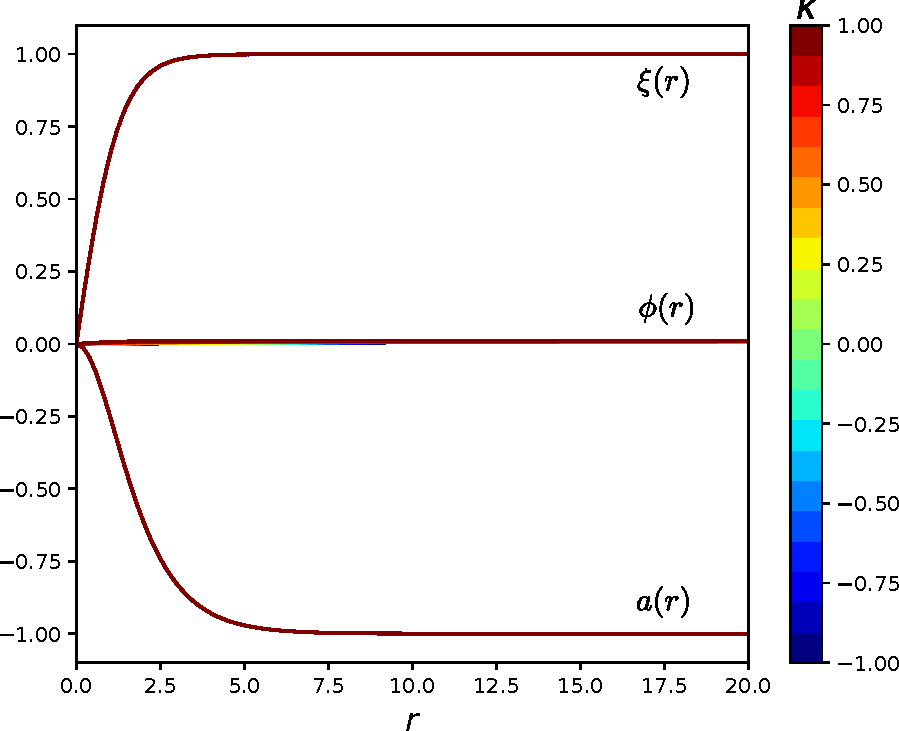
\includegraphics[scale=1]{n1h1np1hp1l1lp1v001vp1edited.pdf}
		\caption{Solutions for $n = h = n' = h'  = \lambda=\lambda' = 1,\ v =0.01,\ v' = 1 $ and $\Delta \kappa = 0.1$, $\kappa^2<1$.}
		\label{fig:sol1}
\end{figure}

\begin{figure}
	\centering
	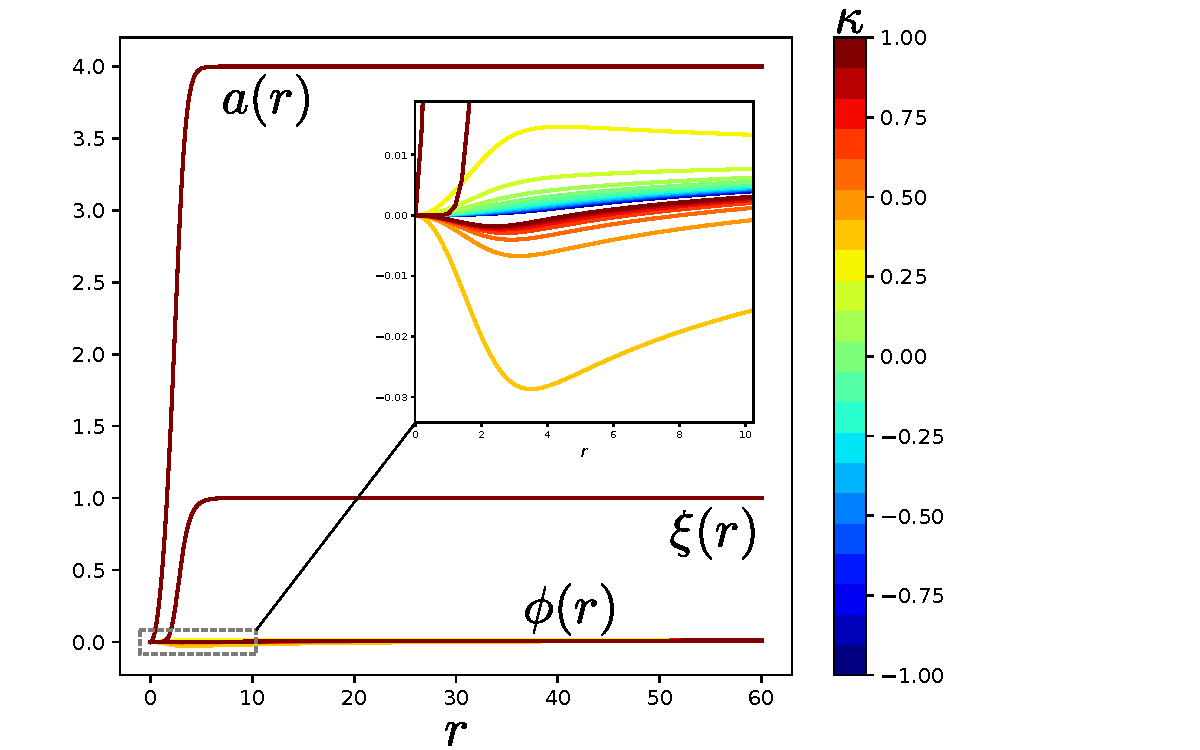
\includegraphics[scale=1]{n-2h05np10hp-25l1lp1v001vp1combined.pdf}
		\caption{Solutions for $n = -2,\ h =0.5,\ n' = 10,\ h' = -2.5,\  \lambda=1,\ \lambda' = 1,\ v =0.01,\ v' = 1 $ and $\Delta \kappa = 0.1$, $\kappa^2<1$.}
		\label{fig:coaxial}
\end{figure}

\begin{figure}
	\centering
	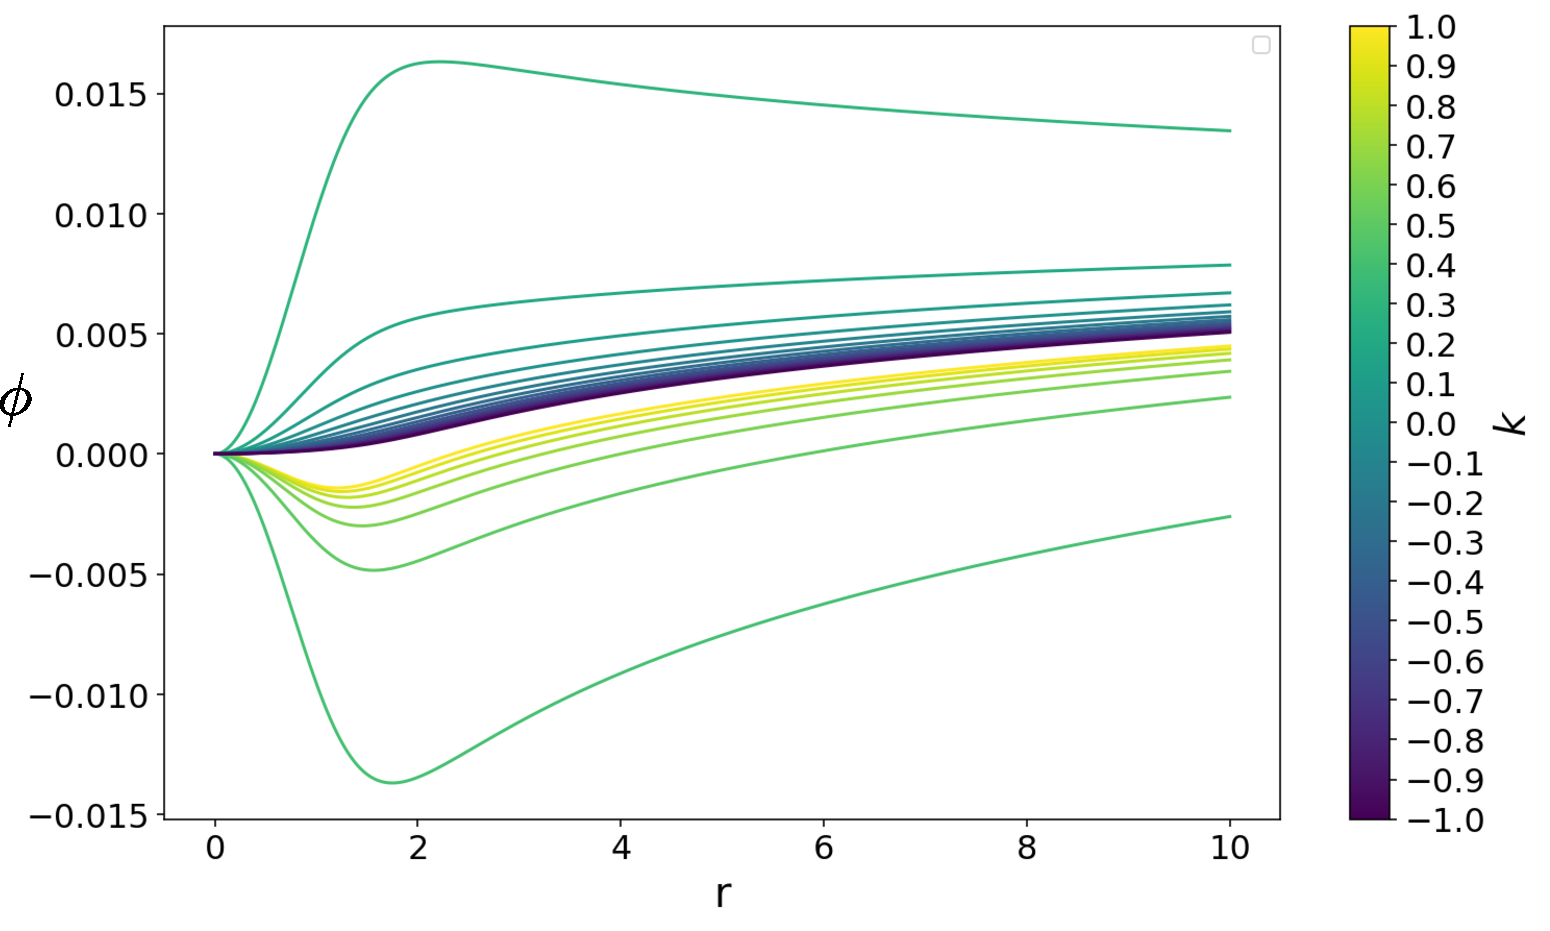
\includegraphics[scale=0.5]{JA1.pdf}
		\caption{Victor's plot: Zoom in, coaxial solutions in the $\phi$ field. With $n = -2,\  h = 0.5,\ n' = -10, h' = 2.5, \lambda=\lambda' = 1,\ v =0.01,\ v' = 2 $ and $\Delta \kappa = 0.1$, $\kappa^2<1$.}
		\label{fig:victor}
		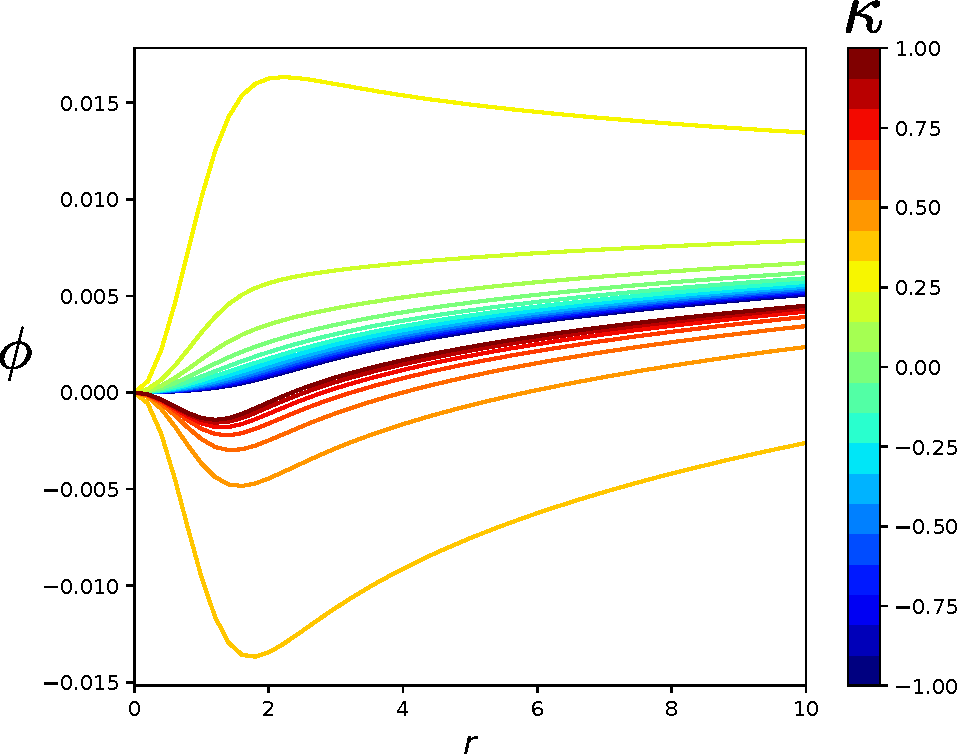
\includegraphics[scale=0.8]{jacoaxial1.pdf}
	\caption{Jose Antonio's plot: coaxial solutions in the field $\phi$. With $n = -2,\  h = 0.5,\ n' = -10, h' = 2.5, \lambda=\lambda' = 1,\ v =0.01,\ v' = 2 $ and  $\Delta \kappa = 0.1$, $\kappa^2<1$.}
	\label{fig:ja}
\end{figure}

\begin{thebibliography}{9}
\bibitem{bogo1975} Bogomoln'yi E. B. The stability of classical solutions. \emph{Sov. J. Nucl. Phys}. 24, (1975) 861-870.

\end{thebibliography}
%Victor's parameters $n = -2,\  h = 0.5,\ n' = -10, h' = 2.5, \lambda=\lambda' = 1,\ v =0.01,\ v' = 2 $.

%Using the dictionary above, Jose Antonio's parameters are $n = -2,\  h = 0.5,\ n' = -10, h' = 2.5, \lambda=\lambda' = 1,\ v =0.01\sqrt{2} \approx 0.014,\ v' = 2\sqrt{2}\approx 2.82 $ and $-0.5<\kappa<0.5$.


%\begin{figure}
%	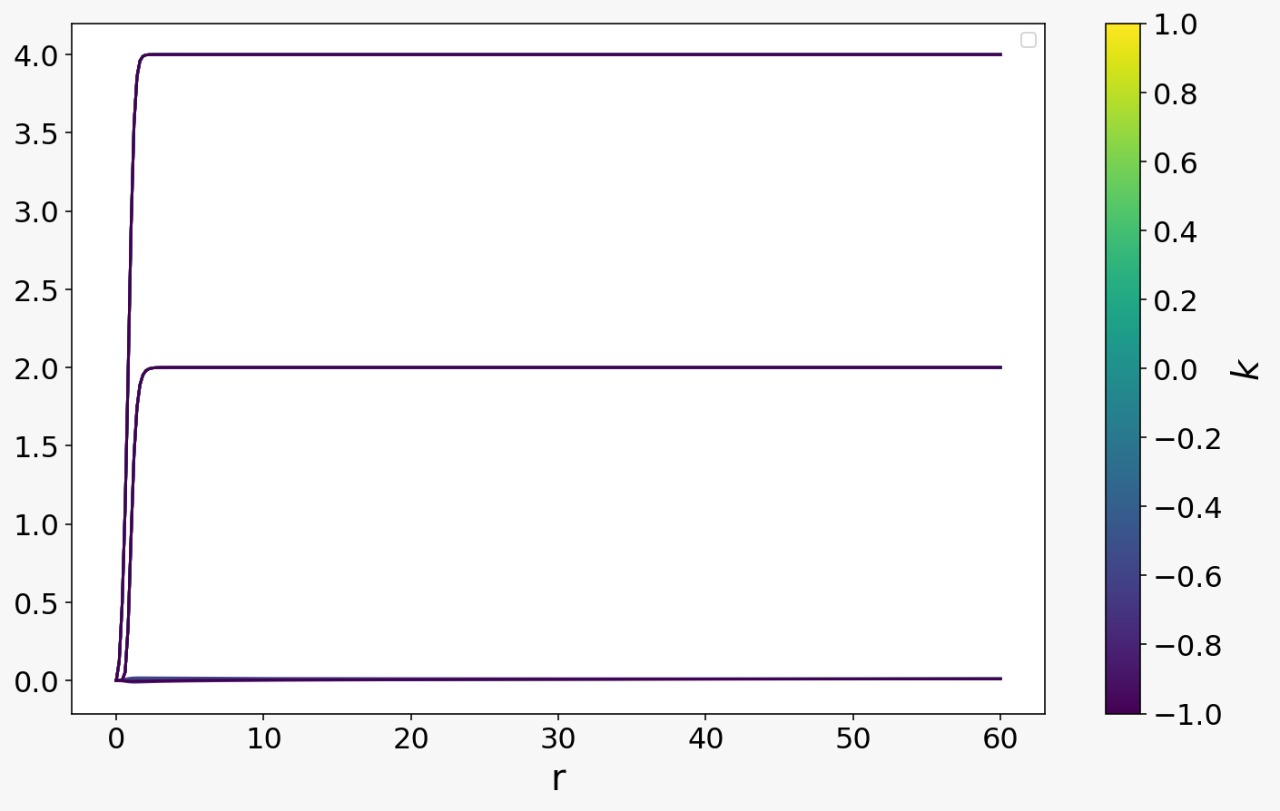
\includegraphics[scale=0.3]{coaxial1.jpeg}
%	\caption{Victor's plot: Zoom out}
%\end{figure}
%
%\begin{figure}
%	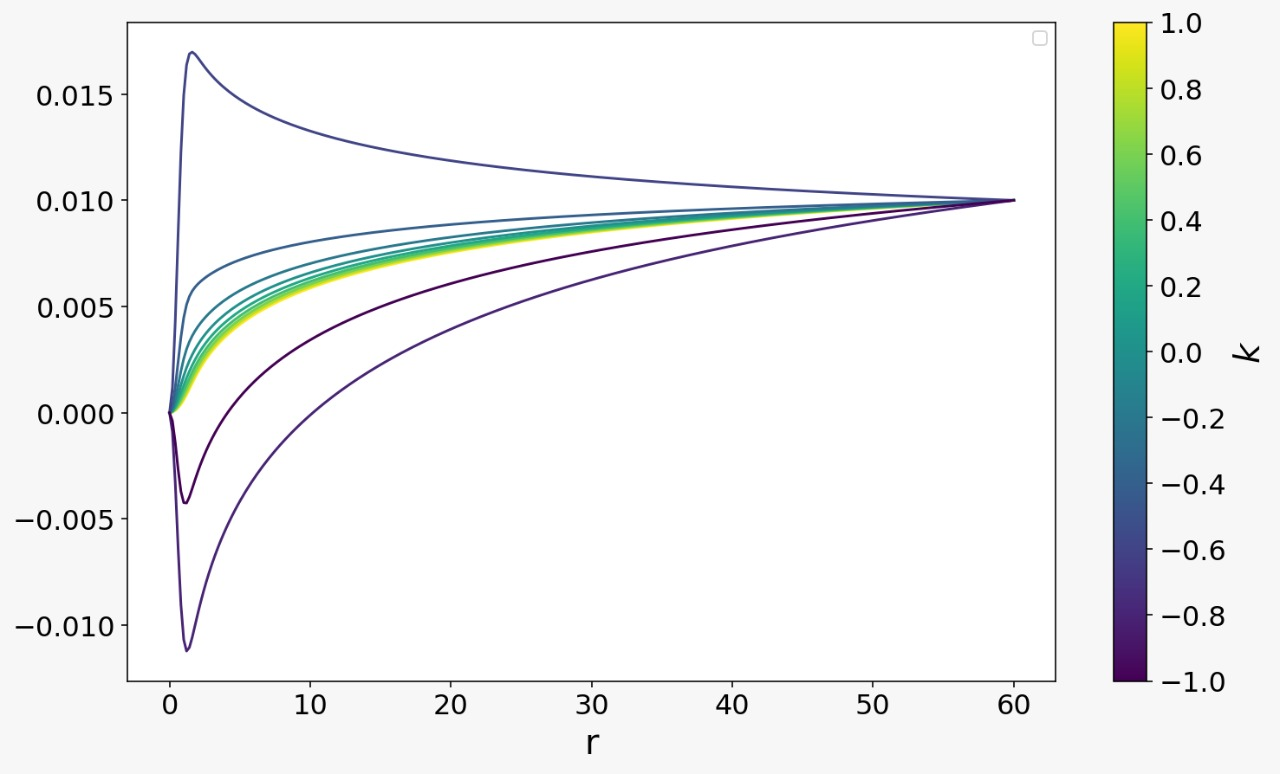
\includegraphics[scale=0.3]{coaxial2.jpeg}
%	\caption{Victor's plot: coaxial solution in the $\phi$ field.}
%\end{figure}
%\begin{figure}
%	\centering
%	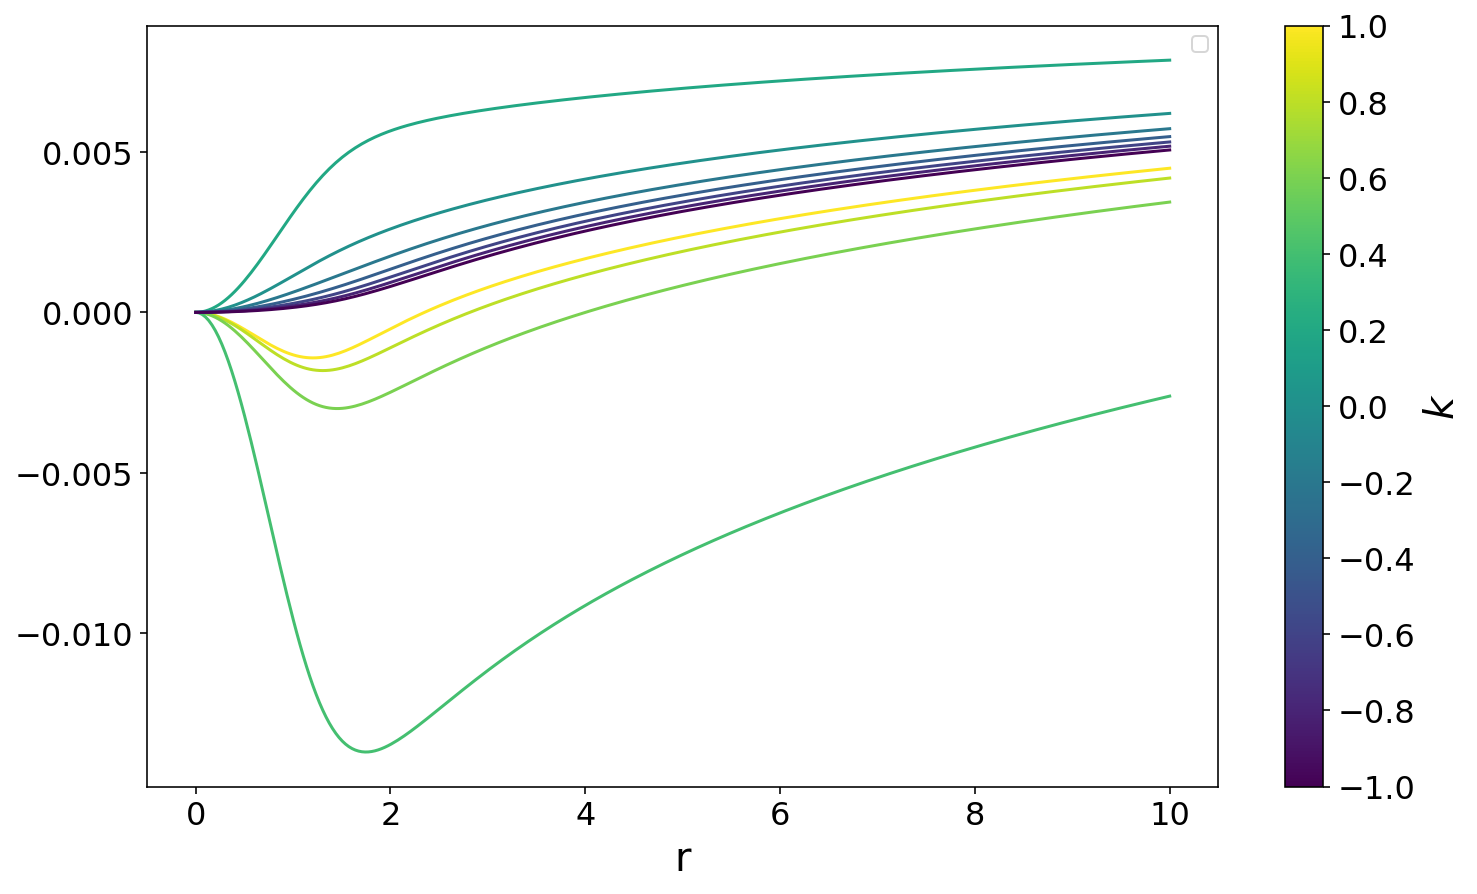
\includegraphics[scale=0.5]{JA2.png}
%		\caption{Victor's plot: Zoom in, coaxial solution in the $\phi$ field. $\Delta \kappa = 0.2$, $\kappa^2<1$}
%		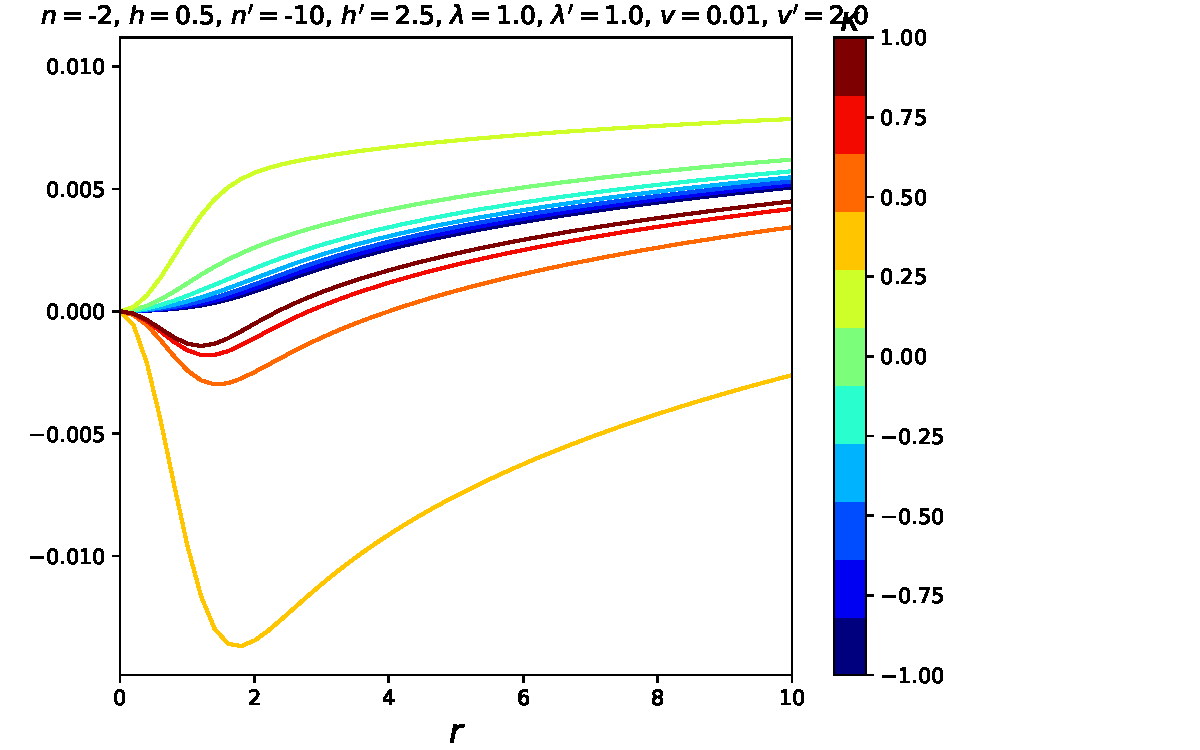
\includegraphics[scale=0.8]{jacoaxial2.pdf}
%	\caption{Jose Antonio's plot: coaxial solution in the field $\phi$. $\Delta \kappa = 0.2$, $\kappa^2<1$.}
%\end{figure}




\end{document}